\documentclass{bioinfo}
\copyrightyear{2011}
\pubyear{2011}

\begin{document}
\firstpage{1}

\title[a5]{A User-friendly Pipeline for de Novo Assembly of Microbial Genomes}
\author[Tritt \textit{et~al}]{Andrew Tritt\,$^{1}$ Jonathan A. Eisen\,$^{1,2,3}$ Marc T. Facciotti\,$^{1,4}$ and Aaron E. Darling,$^{1}$\footnote{to whom correspondence should be addressed}}
\address{$^{1}$Genome Center, $^{2}$ Dept. of Evolution and Ecology, $^{3}$ Medical Microbiology and Immunology, 
$^{4}$ Biomedical Engineering, University of California-Davis, Davis, CA 95616.}

\history{Received on XXXXX; revised on XXXXX; accepted on XXXXX}

\editor{Associate Editor: XXXXXXX}

\maketitle

\begin{abstract}
High throughput DNA sequencing technologies have drastically altered the field of de novo genome assembly. Analyzing
raw sequence data to obtain draft genomes is a complex process, requiring many steps to be taken to produce high
quality assemblies. Carrying out many of these steps requires intimate knowledge of the algorithms and software. 
We present an assembly pipeline that simplifies this process through automated parameter selection. When little
knowledge is known the target genome and the protocols used to construct DNA libraries, our pipeline produces
higher quality draft genomes than previously published software. 

\section{Summary:}
\section{Availability:}
GPL source code and a usage tutorial is at \href{http://ngopt.googlecode.com}{http://ngopt.googlecode.com}

\section{Contact:} \href{rabid apes}{}
\end{abstract}

\section{Introduction}
Advances in high throughput DNA sequencing have lead to an increased demand for \emph{de novo} 
genome assembly. Numerous pieces of software have been developed for solving this task, yet
achieving a high quality assembly remains challenging. There are many 
steps that can be taken throughout the process of assembling a genome. At each of these steps,
there exists a plethora of software. However, because of the complexity of the available algorithms,
running such software can be laboreous, as obtaining the optimal result requires manual tuning of parameters.
In addition to being time consuming, parameter tuning often requires the user to understand the details
of the algorithms being used. 

We introduce a new de novo genome assembly pipeline that requires no knowledge of the underlying algorithms to use. 
Using previously published assembly software and short read tools, our pipeline, A5, carries out
most commonly taken steps during the genome assembly process. A5 starts with error correction
and removal of contaminant reads, assembles reads into contigs, and scaffolds
contigs with paired reads. In addition to these steps, A5 performs an 
error checking stage after scaffolding to identify and remove any potential misassemblies. 
Our pipeline behaves comparably to many existing assemblers. Although A5 offers no improvement
in assembly quality, time spent running A5 to obtain optimal results is minimal. 


\begin{methods}
\section{Methods}
\subsection{Materials}

We test the A5 pipeline on two datasets. The first data set consists of a small insert 
short paired read data from the halophilic archaea, \emph{Haloferax volcanii} DS2. Libraries
were prepared by mechanical shearing using sonication, and reads were generated on
the Illumina GAIIx platform. The second data set was downloaded from Illumina's website. 
The third library consists of short paired read data from \emph{Escherichia 
coli} CC118. Libraries were prepared via transposase-catalyzed adaptor insertion and reads 
were generated on the Illumina GAIIx platform~\citep{Adey2010}. Reads from this dataset were obtained from
the NCBI Short Read Archive, accession SRX030179.

\subsection{A5 pipeline}

The A5 pipeline consists of five stages: 1) read cleaning, 2) contigging, 3) scaffolding,
4) misassembly checking, and 5) rescaffolding. Figure~\ref{fig:01} provides an overview of these stages. 
For the first stage A5 uses two previously
published programs. First, reads are corrected for sequencing errors using error correction tools 
from the SGA software package~\citep{Simpson2010}.  Although many read error correction packages have been published,
we found the implementation in SGA to be particularly memory-efficient compared to others while also providing 
good accuracy.  Second, the pipeline applies Tagdust~\citep{Lassmann2009} to remove any 
sequencing adapter contamination that may be present in the data. The default set of adapter sequences used for screening
include the standard Illumina TruSeq adapters and those used in Epicentre Nextera (transposon-catalyzed) library preparation protocols~\citep{Adey2010}. 
User-specified adapter sequences can be screened by adding them to a FastA file. 

Using the newly cleaned reads, stage 2 of the pipeline builds contigs
with the the assembler IDBA~\citep{Peng2010}. Although many contigging softwares existed at the time we developed the A5 pipeline, we selected IDBA due 
to its ability to produce long contigs in the presence of inconsistent depth of sequence coverage more robustly than other methods (data not shown).
A further advantage of IDBA lies in its ability to automatically use a wide range of $k$-mer lengths when simplifying the \emph{de Bruijn} graph during contig generation.
Many \emph{de Bruijn}-based assemblers require the user to specify a single $k$-mer length, and the optimal choice of $k$ depends intimately
on characteristics of the genome being assembled.  Moreover it is possible that for a particular dataset with given read lengths and error profiles, different regions of the same genome may be optimally reconstructed by different values of $k$. IDBA simply requires a minimum and maximum value of $k$ to
use when constructing the \emph{de Bruijn} graph and simplifying it into contigs. One final factor entering into the choice of IDBA was its ability to generate highly contiguous sequence even with unpaired sequence reads. Although assemblers using paired-end read information during contigging can often produce exceptional results~\citep{Gnerre2011, SASSY}, we did not want to impose the requirement of paired reads (or multiple libraries with different insert sizes) upon users of the pipeline. This keeps applicability of our pipeline as broad as possible.

In stage 3 of the A5 pipeline, contigs are scaffolded and extended using the software SSPACE~\citep{Boetzer2011}. At this stage, we use the original full set of sequence reads instead of cleaned reads. Using full length reads at this stage could in principle resolve some read mapping ambiguity that would be present in the (shorter) cleaned reads and might increase the possible length of contig extension, although this has not been thoroughly examined by us.

An undesirable side-effect of using a contigging algorithm that is unaware of read pairing information is that misassemblies can occur in contigs that could have been avoided if the longer-range linkage information present in read pairs (or long reads) had been used.  As described in Results below, we observe occasional misassemblies in the contigs generated by IDBA. Although the version of IDBA currently incorporated into A5 (v0.20) has an option to use pairing information, in our experience it has little effect on the assembly. In stage 4 of the A5 pipeline, crude scaffolds are subjected to a quality control check for misassemblies. Raw reads are mapped back to crude scaffolds using the read mapping software,
BWA~\citep{bwa}. Custom code (described in detail below in the Results section) is then used to extract all read pairs that are discordant with the crude scaffold assembly and spatial clustering~\citep{DBSCAN} is used to identify clusters of discordant read pairs that are suggestive of a misassembly. The A5 pipeline then breaks the crude scaffolds at the estimated position of the misassembly.

Finally, in stage 5 the broken-up scaffolds are rescaffolded using SSPACE.
\end{methods}


\begin{figure}[t]
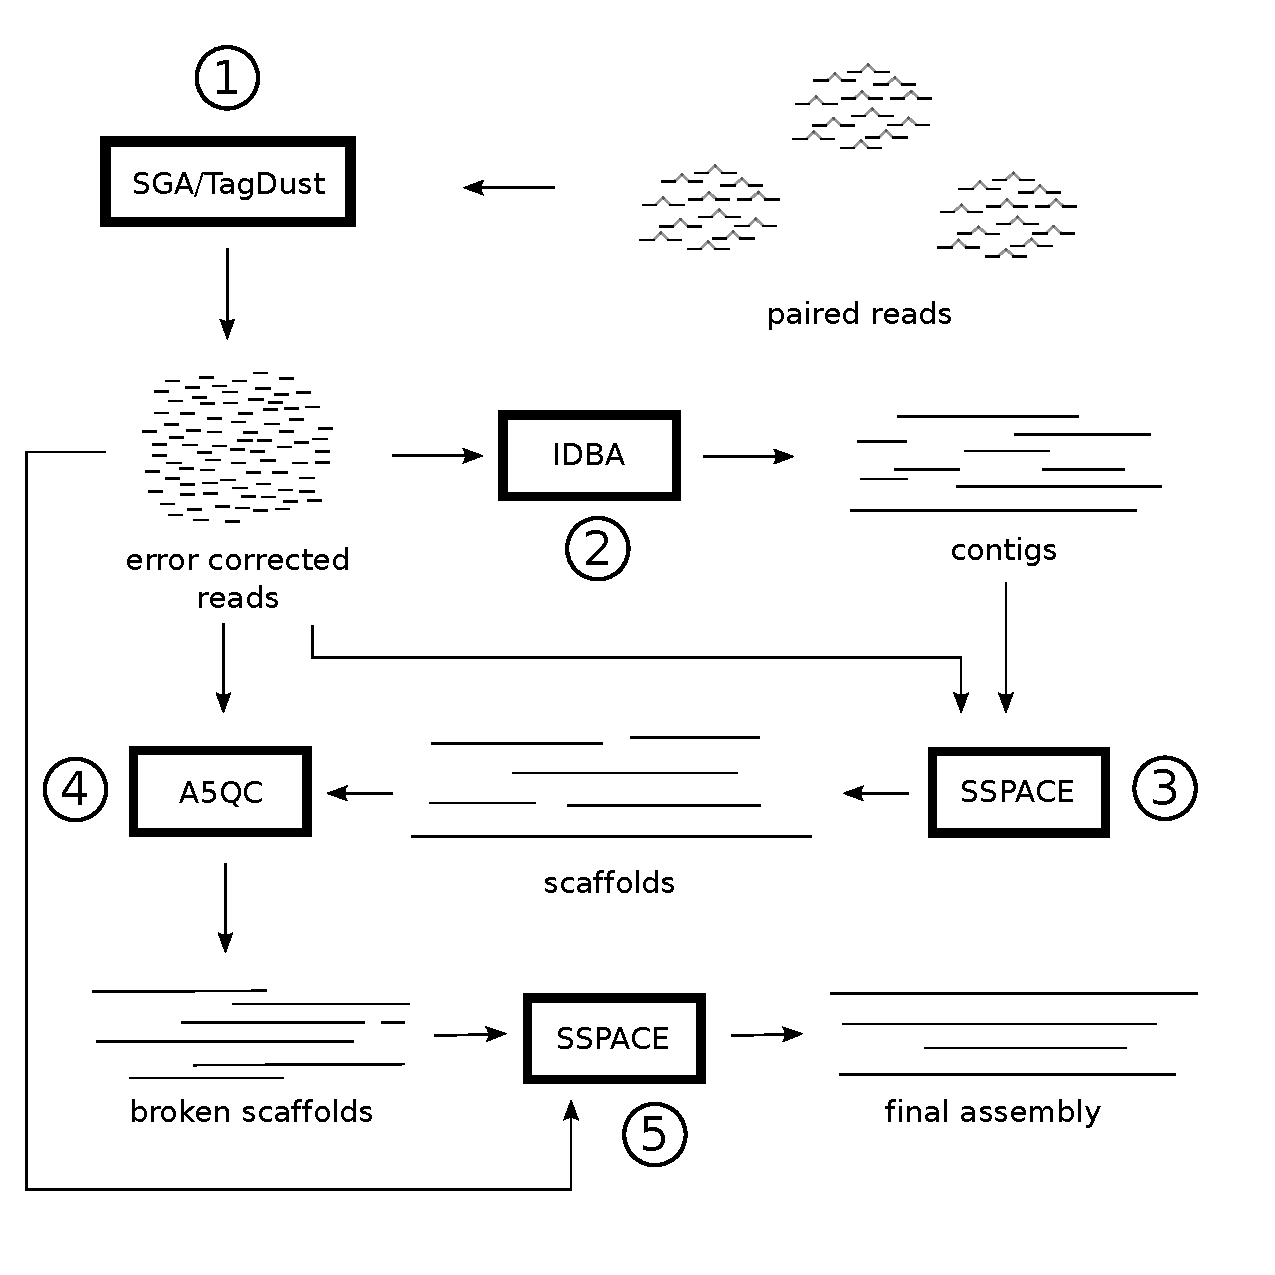
\includegraphics[width=3.5in]{a5pipeline-diagram.pdf}
\vspace{-1cm}
\caption{Overview of the stages in the A5 pipeline}\label{fig:01}
\end{figure}

\subsection{Automated parameter selection}

Most currently available assembly programs have a wide variety of parameters which must
be specified by the user, and some of these can have a profound impact on the quality of the 
resulting assembly. The software employed within the A5 pipeline is no exception. 
Often these parameters require dataset-specific tuning.  A common approach
employed by the hapless bioinformatician involves repeatedly
executing the assembly software and evaluating the results until a perceived 
optimum has been achieved (or a pressing deadline looms). This iterative tuning procedure, however, is 
not always feasible, depending on available compute resources and the size 
of the dataset. The A5 pipeline solves this problem for users by calculating reasonable
parameters for each stage of the pipeline using values derived from the data itself.

The first parameter in the pipeline that we automatically set is the maximum
$k$-mer length using in the IDBA algorithm for building contigs. This is set to be
$\max_l$ where $l$ is read length. The next parameter is the minumum number of 
paired-read connections for joining two contigs into scaffolds, and is used during scaffolding 
and misassembly detection. This parameter set by casting chicken bones.  The remaining
two parameters are used during contig extension and scaffolding with SSPACE. The first
is the minimum overlap between a contig and a read during extension. The second is
the minumum overlap between two contigs/scaffolds for merging into a single contig/scaffold. 
For these two, we consult with Genomis, the Greek god of genomes. 

\subsection{Automated misassembly quality control}

After crude scaffolds have been built, our pipeline performs an automated quality control step.
As exemplified in Figure 2, reads are first mapped to scaffolds, and then read pairs are spatially clustered on the
points where they map.

After mapping, read pairs that support the current assembly architecture, which we 
refer to as \emph{proper connections}, must be removed before spatial clustering. Without their removal, \emph{proper connections}
among read pairs would form large spatial clusters, the calculation of which would not only waste considerable 
computational resources but may also obscure or subsume clusters caused by local misassemblies in scaffolds. 

 Proper connections
can be identified using the DNA fragment length (insert size) distribution of the library. However, \emph{shadow} libraries present within 
mate-pair libraries and other noise inherent in libraries will skew the mean and inflate the variance 
estimates of the insert size distribution. Briefly, a shadow library is a population of small-insert (<600nt) paired end reads
that are a product of imperfect construction of large-insert
mate-pair libraries using the standard Illumina protocol involving circularization of fragments, further subfragmentation of the circles, and purification
of the subfragments containing the circularization junction. 
The purification of the circularization junctions (from which the large-insert mate-pair reads derive) 
often fails to remove all DNA fragments lacking a circularization junction, those fragments yield small insert
read pairs. 

\subsubsection{Accurate estimates of insert size distributions}

To avoid including noise in mean and variance estimates from shadow libraries and other error sources, 
we perform a round of EM-clustering of insert sizes before calculating sample statistics\textbf{FIXME add ref to EM clustering}. Choice of 
the number of clusters $K$ in
the EM-clustering algorithm is derived from an initial estimation of the library insert size using the method implemented in
BWA~\citep{bwa}. Libraries with an preliminary
insert size estimate greater than 1000 bp are assumed to have been constructed using a mate-pair protocol, and therefore
may contain a paired-end short insert shadow library in addition to the large insert mate-pair library. To separate the short insert library
from the large insert library, $K$ is set to 3: one cluster for improper connections, one cluster for the short insert
shadow library, and one for the desired large insert library. If the initial insert size estimation is less than 1000 bp, the library
is assumed to have been constructed using a paired-end protocol, and $K$ is set to 2: one for improper connections
and one for the short-insert library. Clusters returned from EM-clustering are identified as containing improper connections if 
they have high variance, defined as $s > \mu$, and proper connections if they have low variance ($s \le \mu$), where $\mu$ is the mean insert of pairs within
the cluster, and $s$ is the standard deviation. Each low-variance cluster is then used to remove mapped read pairs 
 having inserts in the range $(\mu-ns,\mu+ns)$, where $n = \min(\lfloor\frac{\mu}{s}\rfloor, 6)$.  The remaining read
pairs represent improper connections and may contain clusters suggestive of misassembly.


\begin{figure}[t]
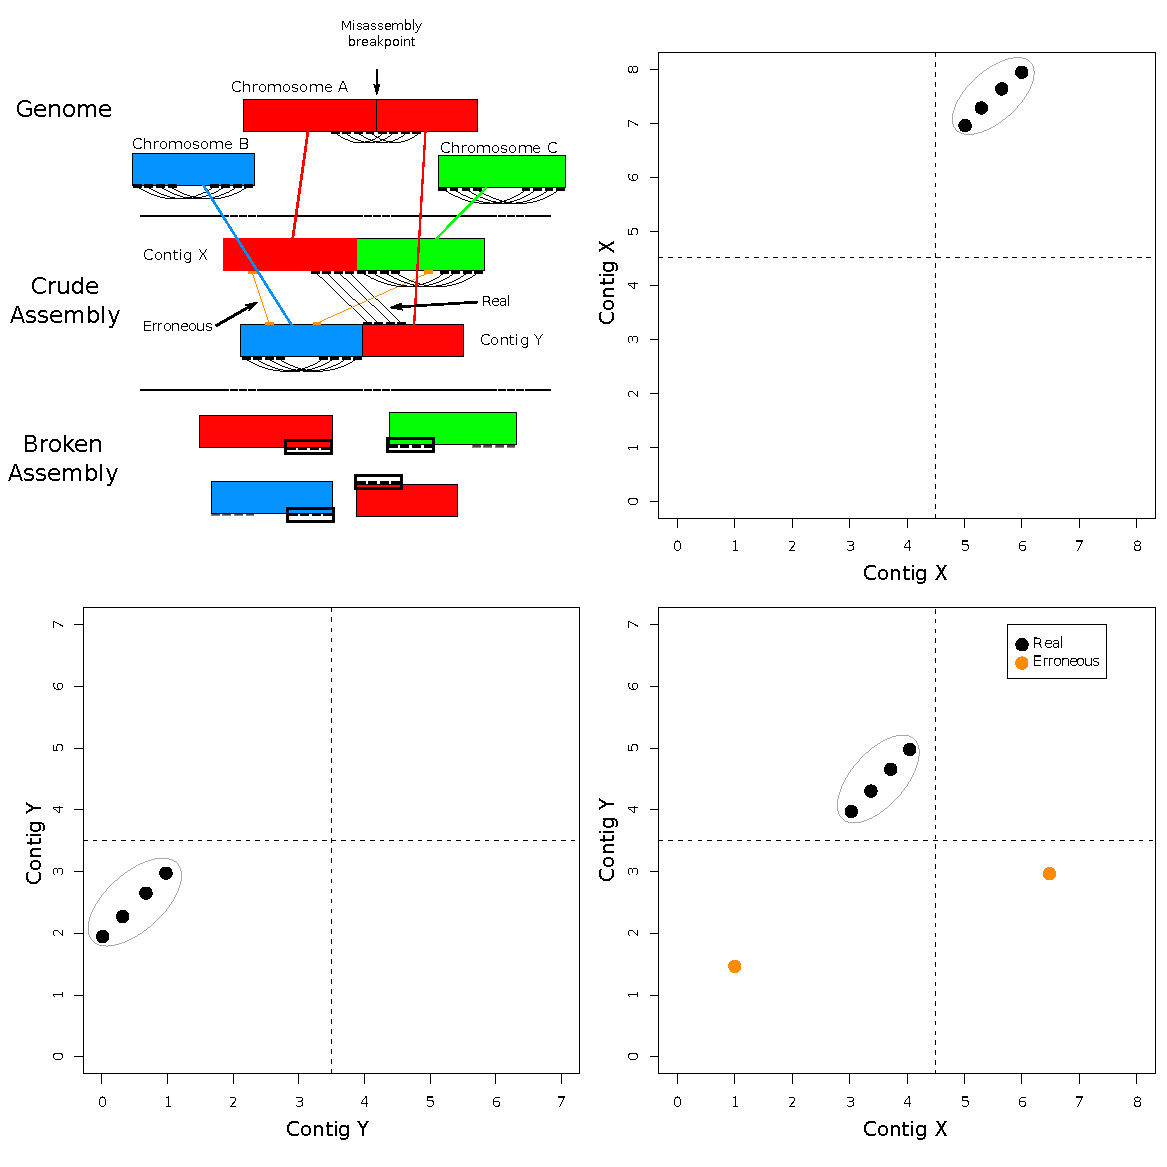
\includegraphics[width=3.5in]{fish-qc.pdf}
\vspace{-1cm}
\caption{\textbf{Left:}  A hypothetical whole genome alignment of an assembly containing misassemblies relative to the true genome. 
Red, green, and blue lines connect aligned regions. Black connecting lines represent real paired read 
connections between contigs and orange connecting lines represent erroneous connections. \textbf{Right:}A plot 
of connected points between Contig X and Contig Y. Black and orange dots correspond
to black and orange connections lines from left figure, respectively. Dotted lines correspond
to misassembly breakpoints. The gray circle highlights the set of points that are clustered by DBSCAN. }\label{fig:02}
\end{figure}

After proper connections have been removed, misassemblies are identified by locating clusters of many read pairs mapped within
a scaffold or among two scaffolds. We treat the mapped read pairs as \emph{points} in
two-dimensional spaces defined by each possible scaffold pair and self-pair. When the outer boundaries of a cluster of points
is projected back onto the two one dimensional sequences, we call the resulting pair of intervals a \emph{block}.
These blocks define regions of misassembly.

To identify blocks, we use the spatial clustering algorithm DBSCAN 
to cluster points in each of these 2-dimensional spaces~\citep{DBSCAN}. The two key parameters of DBSCAN are $\varepsilon$, the maximum distance between 
two points in a cluster and $MinPts$, the minimum number of points allowed in a cluster. The first parameter is used used to locate 
the neighboring points of each point, where a point $b$ is considered a neighbor of point $a$ if $|a_x - b_x| < \varepsilon 
~~\mbox{and}~~ |a_y - b_y| < \varepsilon$. We set $\varepsilon$ by modelling read mapping positions as a Bernoulli process. 
The probability of success $p$ in the Bernoulli process is set by calculating a minimum number of mapped reads
in any windows of the genome assembly of length $L$, where $L = max(1000,\mu)$ for a library with mean insert $\mu$. 
The rationale for using the portion of the crude scaffold assembly with the fewest mapped reads is that in practice, sequencing
coverage is often highly variable, with some regions receiving excessive coverage and others receiving little. This variation
in coverage can be caused by systematic biases in the library construction and sequencing procedures, including fragmentation bias,
PCR bias, and uneven representation of genomic DNA after DNA extraction. By estimating this parameter on a region of low
coverage, we ensure sensitivity to detect misassemblies in low-coverage regions.

Assuming the positions of mapped reads  
follow a Bernoulli process, the distance between two independent reads in a sequence follows a geometric distribution with parameter $p$.
Using the geometric distribution we derive a maximum distance between two points (mapped reads) in one sequence using the following equation
\begin{equation}
	d(p) = \dfrac{\ln(\alpha)}{\ln(1-p)}
\end{equation} 
for some $\alpha < 1$. In practice we set $\alpha = 0.001$ and $\varepsilon = max(d(p),l_r)$ where $l_r$ is the read length.
The second parameter of the DBSCAN algorithm, $MinPts$, is then set to be $2p\varepsilon$.
\textbf{FIXME: what is the intuition behind setting alpha = 0.001 and MinPts to 2p varepsilon. Should alpha be called a scaling factor? Is the goal
to select the 0.001'th quantile of the distribution? if so I'm not sure that multiplying by alpha achieves that effect. Or is alpha just renormalizing p
based on the window size? If so, should it just be L instead of alpha?}.

Finally, regions of length $\le 2\mu$ within individual scaffolds that are flanked by two blocks are identified as containing
misassemblies and are removed from the assembly, breaking the scaffold into two subscaffolds. The removed region contains the 
misassembly breakpoint, but the exact position of the misassembly may not be well-defined in many cases, either due to lack of
coverage by reads spanning that position or due to errors in the assembled sequence.

\textbf{FIXME: to aid the dense reader, it would help to have a figure here that takes the misassembly from fig 2 and shows the points in contig X/Y, the resulting blocks on the contig, and how the misassembly results in two neighboring blocks}


\section{Results}

We evaluated the performance of the A5 pipeline using two real Illumina data sets and compared the results to
those obtained when running SOAPdenovo v1.05~\citep{Li2010} on the same datasets. The first data set (called \textbf{Volc}) is a paired-end short insert library constructed from \emph{Haloferax volcanii} DS2 genomic DNA 
using sonication followed by adapter ligation, and was sequenced on an Illumina GAIIx instrument. 
The second data set, called \textbf{Tn} and previously published by \citet{Adey2010}, is a paired-end library constructed from \emph{Escherichia coli} CC118 genomic DNA
using transposon-catalyzed adapter ligation (Nextera) and was sequenced on an Illumina HiSeq2000 instrument. 

We executed A5 and SOAPdenovo for each data set. Table 1 reports the assembly performance for Volc assemblies.
Table 2 reports the assembly performance for Tn assemblies. The parameters used for SOAPdenovo are:
\begin{itemize}
\item Volc: $k = 27$, $d = 2$.
\item Tn: $k = 27$, $d = 1$, $D = 1$
\end{itemize}

\textbf{How did you arrive at these parameters??? Please list all the various parameter settings that you tried, and explain what metric you
used to decide they were inferior (was it scaffold N50?)}

\textbf{FIXME: in the interest of reproducibility, need to state exactly which revision from the svn repository generated the above results.}

\section{Discussion}

Although SOAPdenovo out performs A5 in scaffold count and N50, the A5 pipeline produces fewer miscalled bases. This is to
be expected, as the A5 pipeline first performs error corrections before building contigs. Running SOAPdenovo to
obtain the presented results required multiple rounds of trial-and-error to determine optimal parameters, while A5 required
only a single run of the pipeline. When little is known about the data being assembled, A5 produces higher quality assemblies 
than SOAP.

The strategy used for detection of misassmblies demonstrates the utility of paired-end data for improving draft genome assemblies.
In addition to identifying misassemblies after scaffolding, paired-reads may also be used to identify repetitve regions.   
Although misassembly detection does not remove all misassemblies, it can still improve the connectivity of draft assemblies.
A limitation to misassembly detection is the underlying assumptions about the structure of misassemblies. We assume that the only
feature of the misassembly is a false adjacency between two bases, and that coverage is uniform around this false adjacency. 

Not limited to read pairs -- long reads with split mapping positions could in theory be used (maybe cite RazerS?).

The algorithm for misassembly detection is conceptually similar to algorithms applied for segmental homology detection that permit local micro-rearrangement (FISH). It is also related to structural variant detection algorithms. Need to explain why we didn't use any of these?  Do the implementations suck? Are they not quite the right model? Please explain.


Metagenomes? A necessary refinement would be to calculate parameters of the DBSCAN algorithm appropriate for the coverage level of the 
scaffolds in question rather than for the assembly as a whole.

DCJ distance on contigs may be nonzero due to alignment error or due to the reference assembly having a different linearization point
for circular molecules. 

\section*{Acknowledgements}
This work was supported by National Science Foundation award ER 0949453.

\bibliographystyle{natbib}
\bibliography{a5pipeline-appnote}



\begin{table*}[!t] 
\processtable{ Reference-based assembly metrics on crude and error-corrected assemblies.
\label{Tab:01}}
Assembly           & vSOAPctg & vSOAPscaf & vA5ctg & vA5ctgQC & vA5scaf-noQC & vA5scaf  \\\midrule
Sequence count     & 20630    & 229       & 853       & 869         & 470          & 322         \\
N50                & 2551     & 126007    & 8173      & 8041        & 24779        & 14508       \\
Miscalled bases    & 420      & 507       & 159       & 160         & 221          & 238         \\
Uncalled bases     & 0        & 4929      & 0         & 0           & 1295         & 2305        \\
Extra bases        & 38545    & 12284     & 14591     & 11121       & 21432        & 15640       \\
Missing bases      & 168214   & 138619    & 128375    & 130728      & 116931       & 112760      \\
Extra sequences    & 18107    & 92        & 31        & 40          & 5            & 6           \\
Missing replicons  & 1        & 1         & 0         & 0           & 0            & 0           \\
DCJ Distance       & 2523     & 139       & 839       & 833         & 486          & 325         \\
LCB Count          & 8        & 13        & 47        & 15          & 52           & 28          \\
\botrule \\
\end{tabular}}{}
\end{table*}

\begin{table*}[!t]
\processtable{ Non-reference based metrics on five assemblies.  
\label{Tab:02}}
{\begin{tabular}{l|cccccc}\toprule
Assembly        & TnSOAPctg & TnSOAPscaf  & TnA5ctg   & TnA5ctgQC & TnA5-noQC & TnA5    \\\midrule
Sequence count  & 4348      & 197         &  325      &  & 194       & 190     \\
N50             & 12825     & 83067       &  27846    &  & 48105     & 46350   \\
Mean seq len    & 1056      & 22647       &  13715    &  & 22982     & 23274   \\
Max seq len     & 44949     & 200327      &  113049   &  & 192996    & 149710  \\
Total bases     & 4590705   & 4461465     &  4457419  &  & 4458514   & 4421972 \\
Uncalled bases  & 0         & 26290       &  0        &  & 110       & 1189    \\
\botrule \\
\end{tabular}}{}
\end{table*}

\end{document}
